% File for libamtrack manual
% Copyright 2006, 2010 Steffen Greilich / the libamtrack team
% This file is part of the libAmTrack project (libamtrack.dkfz.org).

\chapter{Radial dose distributions}
\label{chap:RDDs}

One of the most disputed submodels in AT modelling is the parametrization of the distribution of radial dose around the particle tracks ('radial dose distribution', RDD). Up to now, \la{} can use the RDDs given in Tab. \ref{tbl:RDDs} and Fig. \ref{fig:RDDs}. 


\begin{table}
\label{tbl:RDDs}
\begin{tabular}{m{0.25\textwidth}m{0.60\textwidth}m{0.15\textwidth}}

\hline
\textbf{Name} & \textbf{Expression} & \textbf{Reference} \\
\hline

\begin{center}Test\end{center}&
$d(r)=c\cdot\Theta(-r_{max})$&
\textsl{simple step function}\\

\begin{center}Katz (point target)\end{center}&
$d(r)=\frac{N_e\cdot e^4}{m_e c^2}\cdot\frac{1}{{\rho}_m}\cdot\frac{z^2}{\beta^2}\cdot\frac{1}{\alpha}\cdot\frac{1}{r^2}\cdot (1-\frac{r}{r_{max}})^\alpha=d_{point}(r)$&\cite{Zhang_et_al_1985}\\

\begin{center}Katz (extended target)\end{center}&
$d(r)=\frac{1}{A}\int_{|r-a_0|}^{|r+a_0|}{2\cdot\Phi\cdot\hat{r}\cdot d_{point}(\hat{r})\cdot d\hat{r}}$&\cite{Waligorski_1988}\\

\begin{center}Site\end{center}&
$d(r)=\begin{cases}c&\text{if $r<a_0$,}\\
d_{point}(r)&\text{otherwise.}
\end{cases}$&\cite{Hansen_and_Olsen_1984}\\

\begin{center}Gei{\ss}\end{center}&
$d(r)=\begin{cases}c&\text{if $r<a_0$,}\\
\frac{c}{r^2}&\text{if $a0\le r\le r_{max}$}\\0&\text{if $r>r_{max}$}\end{cases}$&\cite{Geiss_et_al_1997}\\

\hline
\end{tabular}
\caption{RDDs implemented in \la{}.}
\end{table}


\begin{figure*}
	\centering
		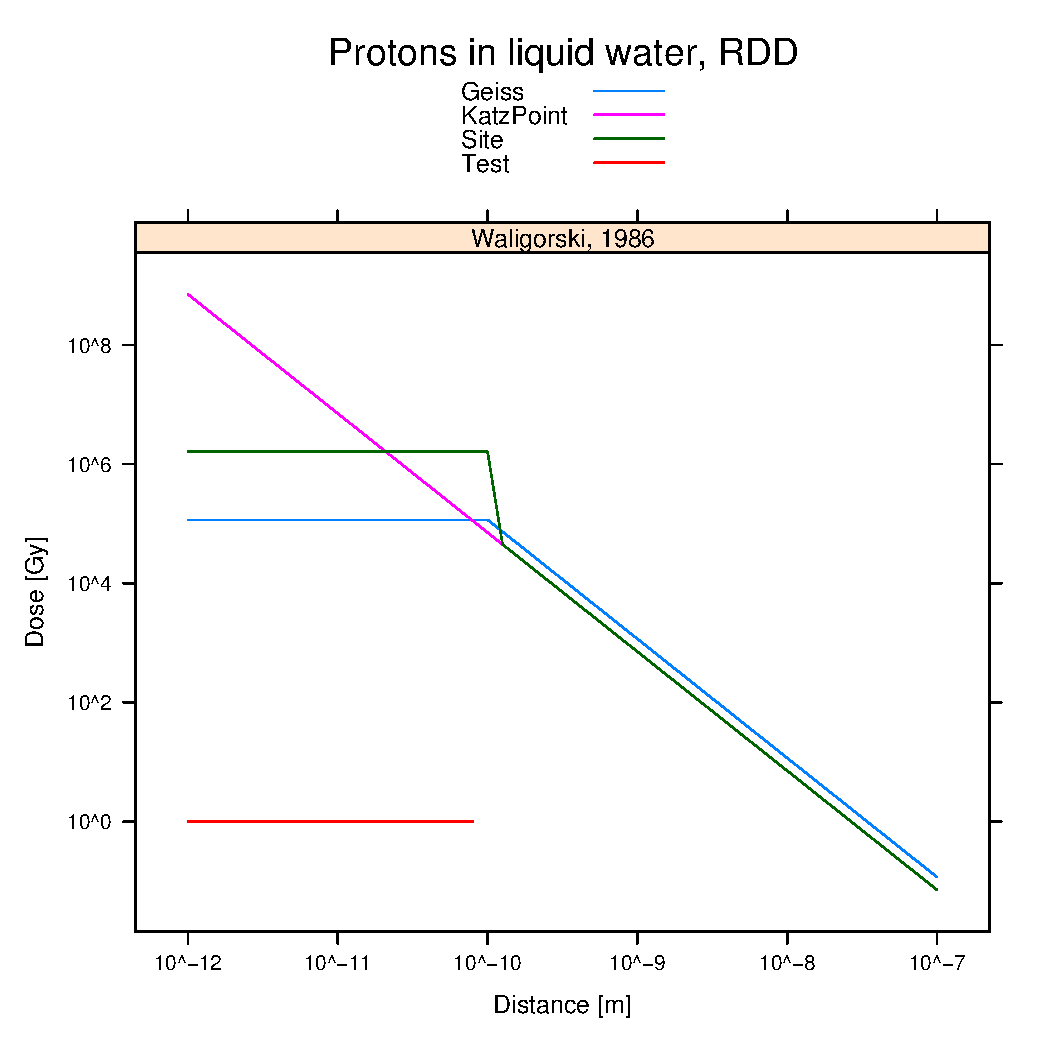
\includegraphics[bb=0 0 2067 1988,width=1.0\textwidth]{pictures/RDD.png}
	\caption{Radial dose distribution submodels available in \la{}}
	\label{fig:RDDs}
\end{figure*}



\section*{Document status}
\begin{tabular}{l l}
2010.06.01&Created by S. Greilich
\end{tabular}